\documentclass[border=15pt, multi, tikz]{standalone}
\usepackage{import}
\usepackage{etoolbox}
\usepackage{graphicx}
\usepackage{svg}
\usepackage{colortbl}

\usetikzlibrary{positioning,matrix,fit}
\usetikzlibrary{3d} %for including external image
\usetikzlibrary{decorations,shapes}
\usetikzlibrary{decorations.shapes}
\usetikzlibrary{decorations.markings}
\usetikzlibrary{decorations.pathreplacing}
\usetikzlibrary{backgrounds}
\usetikzlibrary{calc}
\usetikzlibrary{arrows.meta,arrows}
\graphicspath{{image/}}
\colorlet{cvTestColor}{red!20}
\colorlet{cvValColor}{yellow!20}
\colorlet{cvTrainColor}{green!20}

\begin{document}
  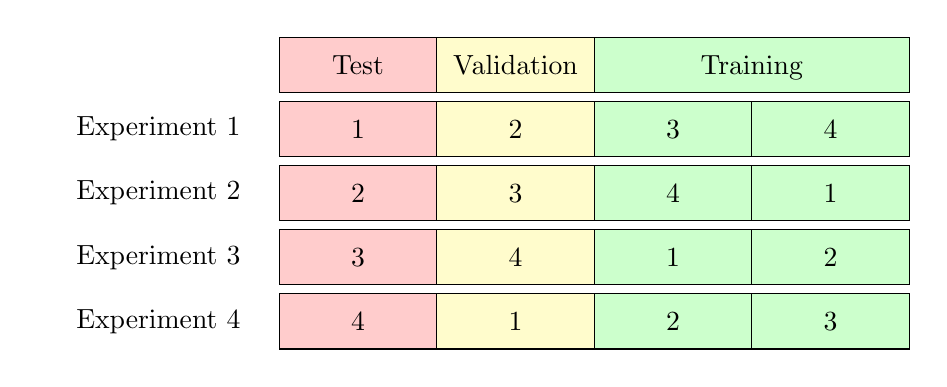
\begin{tikzpicture}
    \matrix (table) [matrix of nodes,
        nodes={minimum height = 7mm, minimum width = 2cm, outer sep=0, anchor=center, draw},
        column 1/.style={nodes={draw=none}, minimum width = 6cm, inner xsep=5mm},
        column 2/.style={nodes={fill=cvTestColor}},
        column 3/.style={nodes={fill=cvValColor}},
        column 4/.style={nodes={fill=cvTrainColor}},
        column 5/.style={nodes={fill=cvTrainColor}},
        row 1 column 4/.style={nodes={draw=none}},
        row 1 column 5/.style={nodes={draw=none}},
        row sep=1mm, column sep=-\pgflinewidth, nodes in empty cells,
        e/.style={fill=yellow!10}
      ]
      {
        & Test & Validation & &\\
        Experiment 1 & 1 & 2 & 3 & 4\\
        Experiment 2 & 2 & 3 & 4 & 1\\
        Experiment 3 & 3 & 4 & 1 & 2\\
        Experiment 4 & 4 & 1 & 2 & 3\\
      };
      \node[fit=(table-1-4)(table-1-5), minimum height = 7mm, minimum width = 2cm, outer sep=0, inner sep=0, anchor=center, draw,  fill=cvTrainColor] (n1) {};
      \node[fit=(n1), yshift=-1.5mm] {Training};
  \end{tikzpicture}
\end{document}